% This file was created by tikzplotlib v0.9.1.
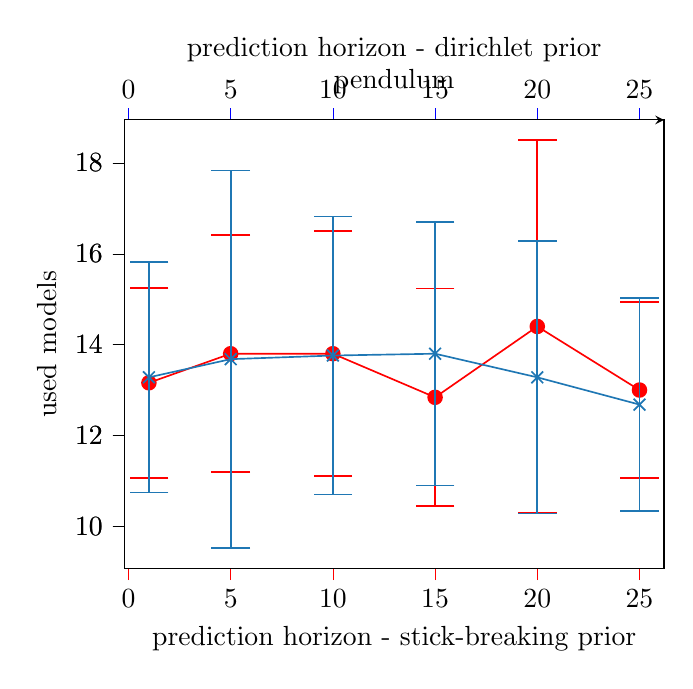
\begin{tikzpicture}

\definecolor{color0}{rgb}{0.12156862745098,0.466666666666667,0.705882352941177}

\begin{axis}[
tick align=outside,
tick pos=left,
title={pendulum},
x grid style={white!69.0196078431373!black},
xlabel={prediction horizon - stick-breaking prior},
xmin=-0.2, xmax=26.2,
xtick style={color=red},
y grid style={white!69.0196078431373!black},
ylabel={used models},
ymin=9.07712288333182, ymax=18.9474306598625,
ytick style={color=black}
]
\path [draw=red, semithick]
(axis cs:1,11.0684933660158)
--(axis cs:1,15.2515066339842);

\path [draw=red, semithick]
(axis cs:5,11.1923190379189)
--(axis cs:5,16.4076809620811);

\path [draw=red, semithick]
(axis cs:10,11.1018524873536)
--(axis cs:10,16.4981475126464);

\path [draw=red, semithick]
(axis cs:15,10.4453392724647)
--(axis cs:15,15.2346607275353);

\path [draw=red, semithick]
(axis cs:20,10.3012196936162)
--(axis cs:20,18.4987803063838);

\path [draw=red, semithick]
(axis cs:25,11.0609280570335)
--(axis cs:25,14.9390719429665);

\addplot [semithick, red, mark=-, mark size=7, mark options={solid}, only marks]
table {%
1 11.0684933660158
5 11.1923190379189
10 11.1018524873536
15 10.4453392724647
20 10.3012196936162
25 11.0609280570335
};
\addplot [semithick, red, mark=-, mark size=7, mark options={solid}, only marks]
table {%
1 15.2515066339842
5 16.4076809620811
10 16.4981475126464
15 15.2346607275353
20 18.4987803063838
25 14.9390719429665
};
\addplot [semithick, red, mark=*, mark size=2.5, mark options={solid}]
table {%
1 13.16
5 13.8
10 13.8
15 12.84
20 14.4
25 13
};
\end{axis}

\begin{axis}[
axis x line=top,
tick align=outside,
x grid style={white!69.0196078431373!black},
xlabel={prediction horizon - dirichlet prior},
xmin=-0.2, xmax=26.2,
xtick pos=right,
xtick style={color=blue},
y grid style={white!69.0196078431373!black},
ymin=9.07712288333182, ymax=18.9474306598625,
ytick pos=left,
ytick style={color=black}
]
\path [draw=color0, semithick]
(axis cs:1,10.7419692673256)
--(axis cs:1,15.8180307326744);

\path [draw=color0, semithick]
(axis cs:5,9.52577323681049)
--(axis cs:5,17.8342267631895);

\path [draw=color0, semithick]
(axis cs:10,10.6969296449477)
--(axis cs:10,16.8230703550523);

\path [draw=color0, semithick]
(axis cs:15,10.9017246507621)
--(axis cs:15,16.6982753492379);

\path [draw=color0, semithick]
(axis cs:20,10.2797333451841)
--(axis cs:20,16.2802666548159);

\path [draw=color0, semithick]
(axis cs:25,10.3353038576395)
--(axis cs:25,15.0246961423605);

\addplot [semithick, color0, mark=-, mark size=7, mark options={solid}, only marks]
table {%
1 10.7419692673256
5 9.52577323681049
10 10.6969296449477
15 10.9017246507621
20 10.2797333451841
25 10.3353038576395
};
\addplot [semithick, color0, mark=-, mark size=7, mark options={solid}, only marks]
table {%
1 15.8180307326744
5 17.8342267631895
10 16.8230703550523
15 16.6982753492379
20 16.2802666548159
25 15.0246961423605
};
\addplot [semithick, color0, mark=x, mark size=3, mark options={solid}]
table {%
1 13.28
5 13.68
10 13.76
15 13.8
20 13.28
25 12.68
};
\end{axis}

\end{tikzpicture}
